We then explore the impact of receive antenna (Rx) and subband on the R-E region for MIMO system with $M = 2$ under a typical FF channel. The dominant eigenvalue of each subband is shown in Figure \ref{fig:mimo-channels}.

\begin{figure}
  \centering
  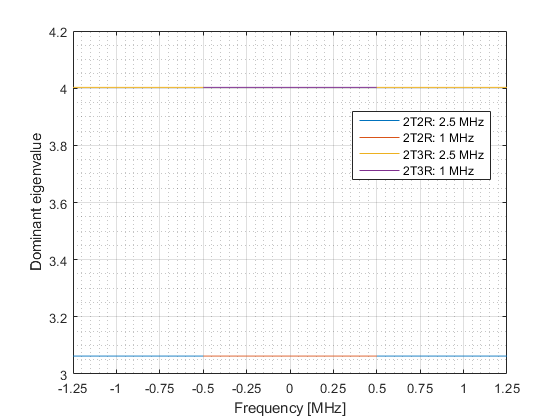
\includegraphics[width=\textwidth]{mimo_frequency_flat_mimo_channel}
  \caption{Frequency response of the MIMO FF channel}\label{fig:mimo-channels}
\end{figure}

\begin{figure}[ht]
  \centering
  \subfigure[FF: $N = 2$]{
    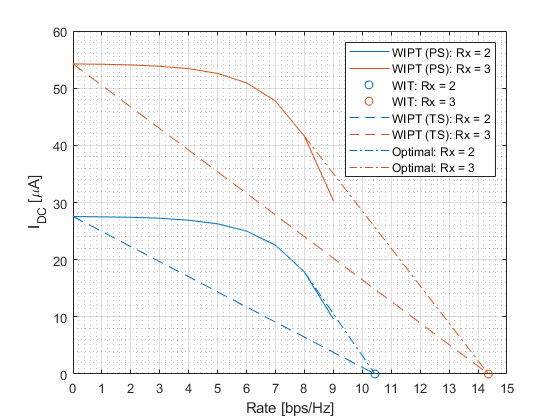
\includegraphics[width=0.48\textwidth]{mimo_re_subband_2}\label{fig:mimo-re-subband-2}}
  \subfigure[FF: $N = 4$]{
    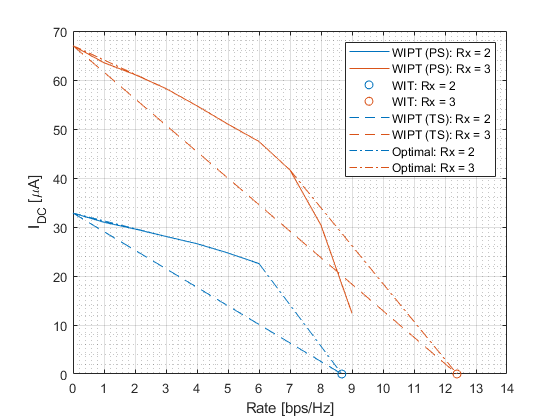
\includegraphics[width=0.48\textwidth]{mimo_re_subband_4}\label{fig:mimo-re-subband-4}}
  \caption{R-E region vs $N$ and $U$ for MIMO FF channels}
  \label{fig:re-mimo}
\end{figure}

As illustrated in Figure \, a contrast between $U = 2$ and 3 suggests that increasing Rx may boost the rate and energy simultaneously, thanks to the multiplexing gain of MIMO. The reason is that for a fixed $M = 2$, increasing $U$ from 2 to 3 provides no extra streams for transmission but leads to a larger eigenvalue of channel matrix, which benefits the R-E region by increasing the effective subband amplitude.

On the other hand, a large $N$ amplifies the harvested power thanks to the rectifier nonlinearity. It can be observed that the R-E curves begin to show some concavity-convexity for $N = 4$, which was first observed for $N = 8$ in SISO channels. A possible reason is that with the aforementioned configuration, each subchannel has 2 virtual streams so that the equivalent subband is indeed $4 \times 2 = 8$. Therefore, MIMO demonstrates a twofold benefit in rate and energy, which requires a smaller $N$ to achieve a certain output power level and is more suitable for low-PAPR systems.

Despite as expected, the conclusions require more evidence since only one specific channel is investigated in the simulation. An averaged result over numerous realizations as in section \ref{sec:mimo} can be more persuasive.

The main problem of Figure \ref{fig:re-mimo} is that the rightmost points of the R-E curves do not reach the x-axis. It results from the discrete rate constraints employed in the simulation. With a step of 1 bps/Hz, the points tend to locate near the integer rates. For instance, the plot corresponding to $U = 2$ and $N = 4$ terminates at a rate of 6 bps/Hz with an output current of \SI{22}{uA}, since proposed PS-WIPT strategy cannot achieve the next rate milestone of 7 bps/Hz. The reason is that the suboptimal phases ${{\mathbf{\Phi }}_P^\prime ,{\mathbf{\Phi }}_I^\prime }$ are determined before the optimization so that the algorithm cannot reach the channel capacity corresponding to WIT. In other words, the GP approach is suboptimal for MIMO systems. 

For a fixed $M$ and $U$, a good R-E tradeoff can be obtained by a combination of the following strategies. In the low-rate region, PS-WIPT is optimal for small $N$ and TS between WPT and WIPT is optimal for large $N$. As rate requirement increases, PS-WIPT can generally guarantee a decent performance on both rate and energy. When the rate constraint is high, TS between WIT and WIPT is the best strategy to enjoy the benefit of multisine and avoid the rate loss of suboptimal phases. 